\section{Durchführung}
\label{sec:Durchführung}

Vor Beginn des eigentichen Versuchs müssen vorbereitende Justierungen durchgeführt werden. Beide Schwingkreise müssen 
auf die gleiche Resonanzfrequenz eingestellt werden.
Dabei wird, wie in Bild \ref{fig:Bild5} dargestellt, eine variierbare Kapazität in einen der Schwingkreise geschaltet. Über eine
Oszilloskop im XY-Betrieb können Lissajous-Figuren dargestellt werden. Es gilt den verstellbaren Kondensator so zu justieren, sodass die beobachtbare
Lissajous-Figur verschwindet. In der Praxis gestalltet sich das auf Grund von unzureichend genauen Justiermöglichkeiten relativ schwierig. Durch eine möglichst gute Minimierung der von der Figur berandeten Fläche kann
ebenfalls in guter Näherung die Resonanzfrequenz gefunden werden. 

\begin{figure}
\label{fig:Bild5}
    \centering
    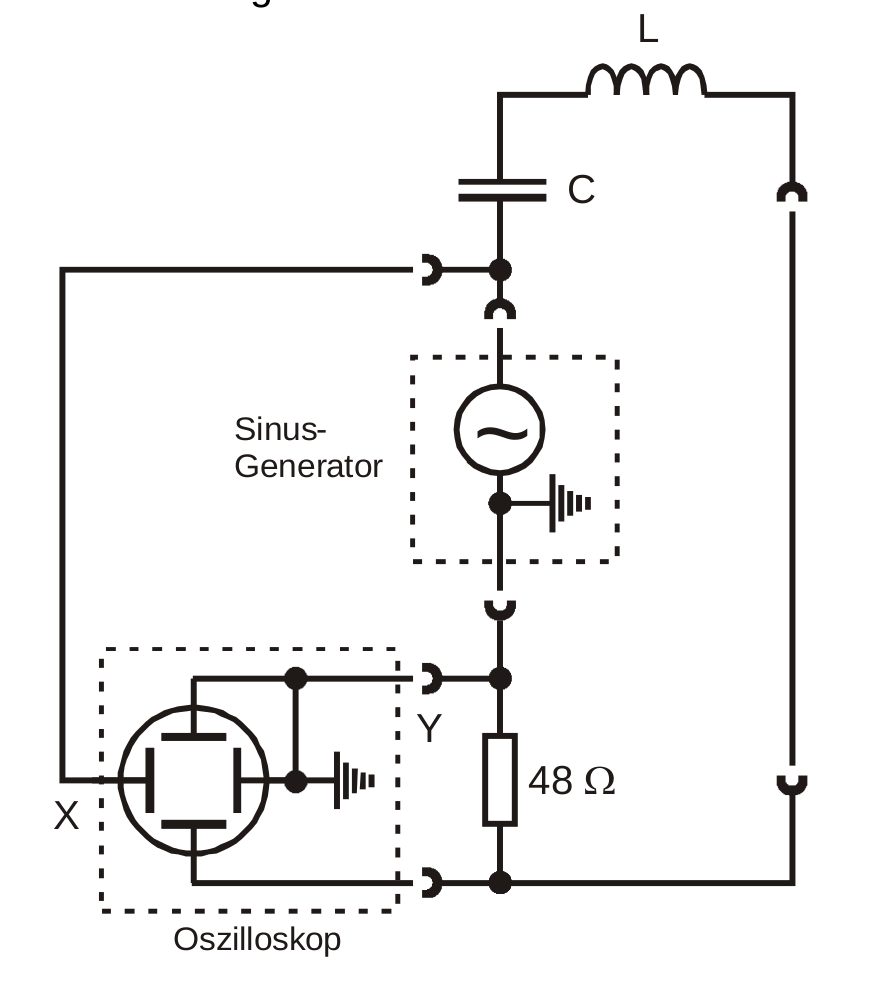
\includegraphics[height=6.0cm]{data/Bild5.png}
    \caption{Schaltbild zur Bestimmung der Resonanzfrequenz eines Schwingkreises.}
\end{figure}

Der Versuch soll mit Hilfe von Schwebungen den Energieaustausch zwischen den beiden Schwingkreisen darstellen.
Dafür wird die Schaltung nach Abbildung \ref{fig:Bild6} aufgebaut. Es ist zu Beachtem, dass nur der linke Schwingkreis durch einen Sinusgenerator angeregt wird.
Mit Hilfe eines Oszilloskops können bei Variation des 
Kondensators $C_K$ verschiedene Schwebungen beobachtet werden. Die Kapazität wird dabei bei von $2\si{\nano\farad}$  bis $2\si{\nano\farad}$
schrittweise erhöht. Jedesmal wird anschließend das Verhältnis der beiden Frequenzen ermittelt, indem die Anzahl der Schwingungsmaxima innerhalb einer Schwebungsperiode 
gezählt werden.



Der zweite Teil des Versuchs zielt auf des ermitteln der Fundamentalschwingungen ab. Die Schaltung wird, bis auf das ersetzten des Rechteckgenerators in
einen Sinusgenerator, so wie in Abbildung \ref{fig:Bild6} beibehalten. Die Generatorspannung soll dabei auf den X-Eingang gegeben werden.
Durch erneute Einstellung des XY-Betriebes können wieder Lissajous-Figuren beobachtet werden. Der Kondensator $C_K$ wird wieder schrittweise verändert und jedesmal die Frequenzen ermittelt, bei 
denen die Lissajous-Figur verschwindet. 


\begin{figure}
\label{fig:Bild6}
    \centering
    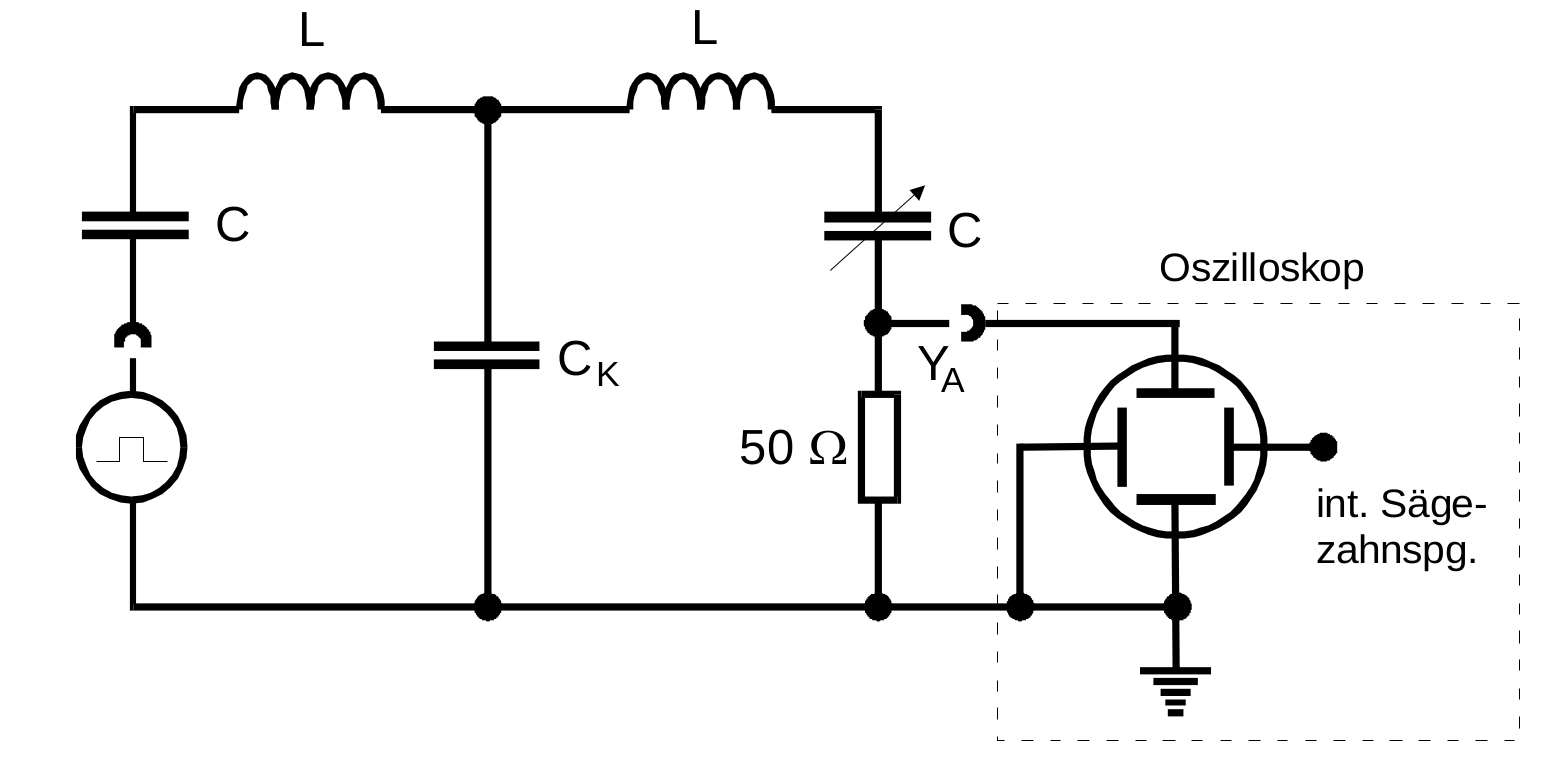
\includegraphics[height=6.0cm]{data/Bild6.png}
    \caption{Schaltbild zur Bestimmung der Fundamentalschwingungen eines gekoppelten Systems.}
\end{figure}





%Was wurde gemessen bzw. welche Größen wurden variiert?